\chapter{Landasan Teori}

\section{Tinjauan Pustaka}
Penelitian ini menggunakan beberapa teori dasar supaya memperjelas proses penelitian dan memberikan pemahaman lebih lanjut. Teori-teori dasar yang berhubungan dan digunakan dalam penelitian adalah sebagai berikut.

\subsection{Konsep \textit{Big Data}}
\textit{Big Data} biasanya sering didefinisikan bersama dengan kompleksitas suatu data \cite{barosenAnalysisComparisonInterfacing2018}. Berbeda dengan tradisional data, \textit{Big Data} merujuk pada pertumbuhan data dalam berbagai format, baik dari struktur, semi-terstruktur, dan tidak terstruktur \cite{oussousBigDataTechnologies2018}. \textit{Big Data} memiliki banyak jenis sehingga membutuhkan teknologi yang lebih bertenaga serta algoritma yang lebih canggih. Pendekatan teknologi yang sering digunakan oleh \textit{Business Intelligence} biasanya tidak dapat lagi efisien jika digunakan.

\textit{Big Data} biasanya didefinisikan menjadi tiga karakteristik (3V), yaitu \textit{Volume, Velocity}, dan \textit{Variety} \cite{furhtIntroductionBigData2016}. \textit{Volume} berkaitan dengan jumlah data yang terbentuk atau dibuat secara terus menerus oleh beragam  perangkat, seperti telepon genggam dan aplikasi (sosial media, sensor, IoT). Jumlah data diharapkan tumbuh 5x lipat pada tahun 2020 \cite{furhtIntroductionBigData2016}. Selanjutnya, \textit{Velocity} memberikan makna bahwa data bertumbuh secara cepat dan harus diproses secara cepat juga untuk memberikan informasi yang berguna \cite{sandhuBigDataCloud2022}. YouTube adalah ilustrasi yang tepat untuk menggambarkan bagaimana pertumbuhan data begitu cepat. Terakhir, \textit{Variety} berkaitan dengan variasi sumber dan format data. 

Penerapan dari \textit{big data} tidak hanya terbatas pada pengumpulan dan penyimpanan data, tetapi juga meliputi analisis dan pengolahan data tersebut untuk menghasilkan wawasan yang berguna. Beberapa sektor yang telah menerapkan \textit{big data} secara luas meliputi kesehatan, keuangan, ritel, dan pemerintahan \cite{oussousBigDataTechnologies2018}. Dalam sektor kesehatan, \textit{big data} digunakan untuk menganalisis informasi pasien secara massal guna meningkatkan kualitas perawatan dan menemukan pola-pola penyakit. Sementara itu, di sektor keuangan, big data membantu dalam analisis risiko, deteksi penipuan, dan personalisasi layanan untuk pelanggan.

\begin{figure}[h!]
    \centering
    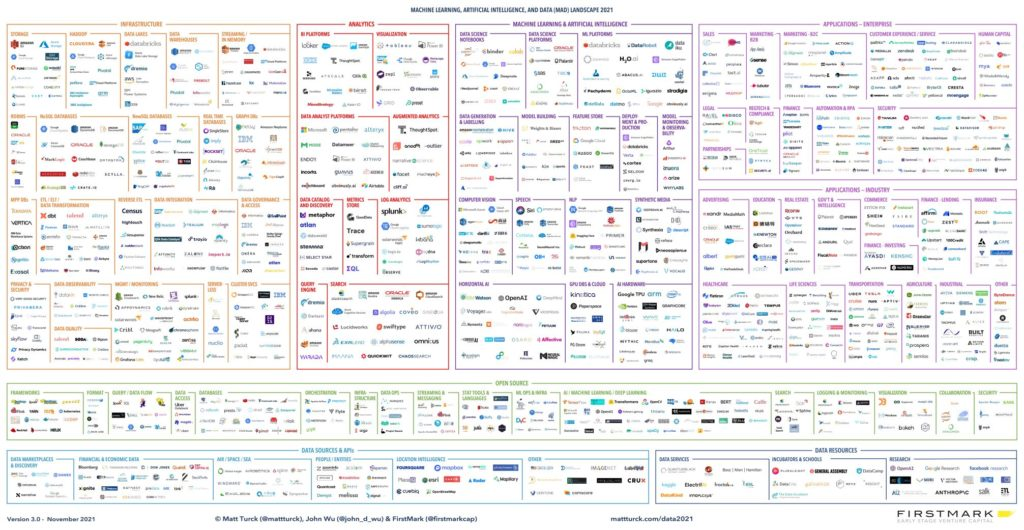
\includegraphics[width=1\textwidth]{figures/ch02/data-stack.jpg}
    \caption{Beberapa Alat di Dunia Data \cite{RedHot20212021}}
    \label{fig:data-stacks}
\end{figure}

Perkembangan alat dalam \textit{big data} juga sangat pesat seperti pada Gambar \ref{fig:data-stacks}. Salah satu contoh signifikan adalah penggunaan teknologi \textit{machine learning} dan \textit{artificial intelligence} (AI) dalam pengolahan data. AI dan \textit{machine learning} memungkinkan analisis data yang lebih akurat dan cepat, bahkan dengan volume dan variasi data yang sangat besar. Alat seperti Hadoop dan Spark telah menjadi standar dalam industri untuk mengelola dan memproses data besar. Selain itu, penggunaan \textit{cloud computing} dalam \textit{big data} memungkinkan penyimpanan dan pengolahan data dalam skala yang lebih besar dan lebih fleksibel.

\subsection{MapReduce}
MapReduce adalah model pemrograman dan implementasi teknik pemrosesan data berukuran besar yang pertama kali dipopulerkan oleh Google pada tahun 2004\cite{kaliaAnalysisHadoopMapReduce2021}. MapReduce menawarkan pemrosesan data yang dapat diandalkan serta \textit{fault-tolerant manner} (tahan terhadap kesalahan).  MapReduce berjalan secara paralel dan berada pada lingkungan komputasi terdistribusi \cite{cTaskFailureResilience2020}. Model ini mengadopsi arsitektur tersentraliasi, yaitu satu \textit{node} berperan sebagai \textit{master} dan \textit{node} yang lain berperan sebagai \textit{workers} atau \textit{slave} \cite{herodotouHadoopPerformanceModels2011, bakratsasHadoopMapReducePerformance2018}. \textit{Master node} bertanggung jawab untuk melakukan penjadwalan kerja, dan \textit{slave node} berperan untuk menjalankan eksekusi kerja. 

\begin{figure}[h!]
    \centering
    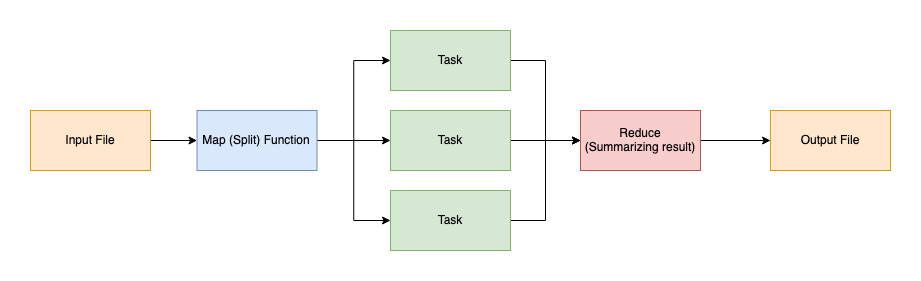
\includegraphics[width=1\textwidth]{figures/ch02/mapreduce-scheme.png}
    \caption{Cara Kerja MapReduce}
    \label{fig:mapreduce-flow}
\end{figure}

MapReduce terdiri dari fungsi \textit{Map} dan fungsi \textit{Reduce} \cite{gandomiHybSMRPHybridScheduling2019}. Kedua fungsi ini tersebar di seluruh \textit{slave node} yang terhubung dalam klaster dan berjalan secara paralel. Fungsi \textit{Map} berperan untuk membagi masalah besar menjadi masalah yang lebih kecil dan mendistribusikannya ke \textit{slave node}. Hasil pemrosesan dari \textit{slave node} akan dikumpulkan oleh \textit{master node} melalui fungsi \textit{Reduce}. Sesuai dengan Gambar \ref{fig:mapreduce-flow}, hasil dari proses \textit{Reduce} yang akan dikirimkan sebagai hasil akhir proses MapReduce.  

Implementasi MapReduce pada \textit{Word Count}\cite{KOMPARASIKECEPATANHADOOP} dapat dilihat pada Gambar \ref{fig:mapreduce-wordcount}. Pada proses MapReduce, data masukan akan melalui beberapa tahapan pemrosesan. Pertama, data akan dipecah menjadi bagian-bagian yang lebih kecil pada proses pemecahan data masukan (\textit{splitting}). Dalam kasus Hadoop MapReduce, data idealnya akan dipecah menjadi beberapa blok berukuran maksimal 128MB.

\begin{figure}[h!]
    \centering
    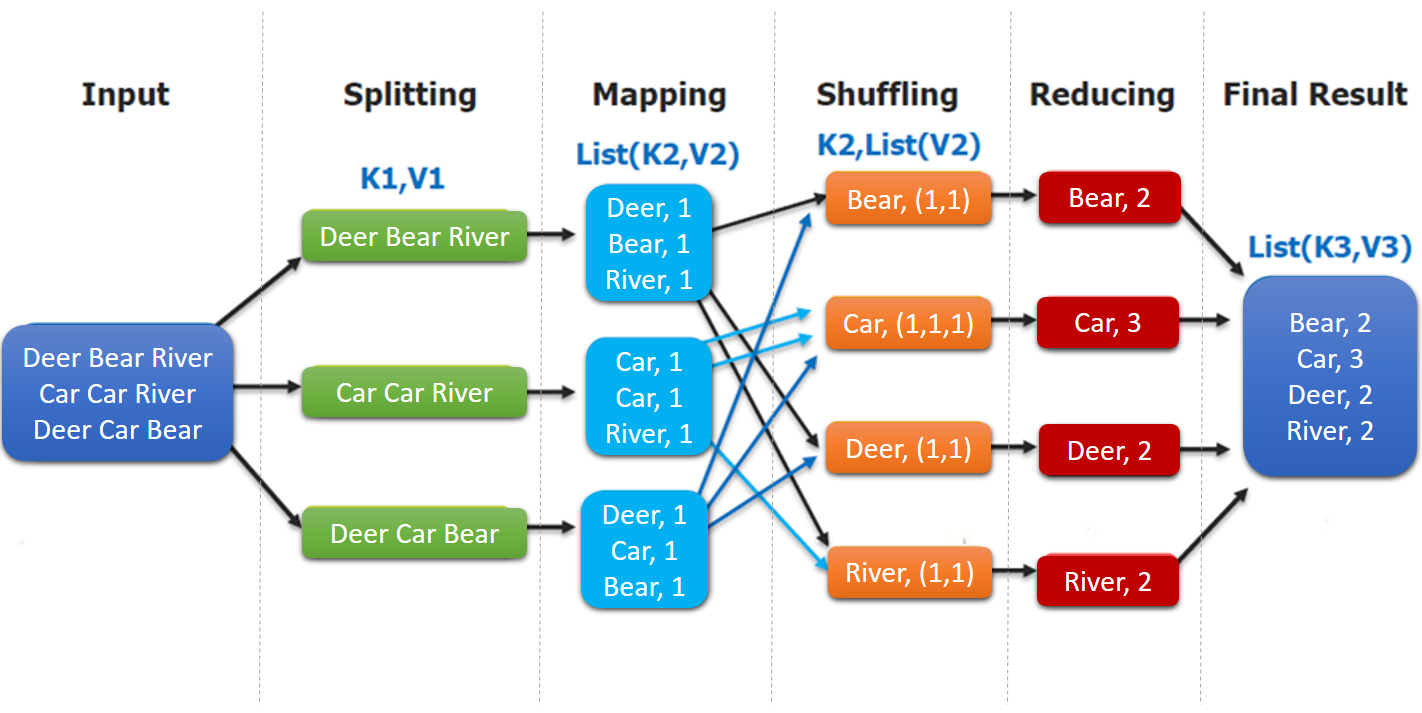
\includegraphics[width=0.9\textwidth]{figures/ch02/map-reduce-word-count-oreilly.png}
    \caption{Implementasi MapReduce pada Word Count \cite{MapReduceDistributedComputing}}
    \label{fig:mapreduce-wordcount}
\end{figure}

Kemudian, blok data tersebut akan diproses lebih lanjut pada tahap pemetaan (\textit{mapping}). Pemetaan merupakan salah satu tahapan terpenting dalam MapReduce. Pada tahap ini, blok data yang sudah dipecah akan diproses untuk menghasilkan pasangan kunci-nilai (\textit{key-value pairs}) sementara, seperti pada contoh kasus \textit{wordcount} yang menghasilkan pasangan kunci-nilai \textit{Dear:1, Bear:1, dan River:1}. Pemetaan dapat melibatkan satu atau beberapa mesin pekerja (\textit{worker}) yang memproses blok data secara paralel.

Selanjutnya adalah tahap pengocokan (\textit{shuffling}) di mana pasangan kunci-nilai hasil pemetaan yang tersebar di beberapa mesin akan dikumpulkan berdasarkan kesamaan kuncinya agar bisa diproses lebih lanjut. Misalnya semua pasangan dengan kunci \textit{Bear} dikumpulkan dalam satu mesin.

Pada tahap terakhir yaitu pengurangan (\textit{reducing}), dilakukan agregasi terhadap pasangan kunci-nilai dengan kunci yang sama untuk menghasilkan keluaran akhir. Seperti pada contoh kasus \textit{wordcount}, pasangan \textit{Bear:1} dan \textit{Bear:1} akan dijumlahkan menjadi \textit{Bear:2} oleh proses pengurangan.

\subsection{Apache Hadoop}
Apache Hadoop adalah perangkat lunak sumber terbuka yang ditulis dengan bahasa pemrograman Java untuk pemrosesan dan penyimpanan data menggunakan komputasi terdistribusi (\cite{ApacheHadoop}). Hadoop dapat diinstalasi pada satu \textit{node} komputer, atau ratusan \textit{node} komputer yang digabungkan dalam sebuah klaster (\cite{maneasEvolutionHadoopDistributed2018}). Berkaitan dengan pemrosesan data, Hadoop mengimplementasikan model MapReduce untuk pemrosesan data secara paralel dan cepat. Selain itu, Hadoop menyediakan sistem penyimpanan data terdistribusi yang dikenal sebagai Hadoop Distributed File System (HDFS) untuk akses data, pemrosesan, dan komputasi \cite{dabasAnalysisCommentsYoutube2019}. Arsitektur Hadoop secara umum dapat dilihat pada Gambar \ref{fig:hadoop-str}.

\begin{figure}[h!]
    \centering
    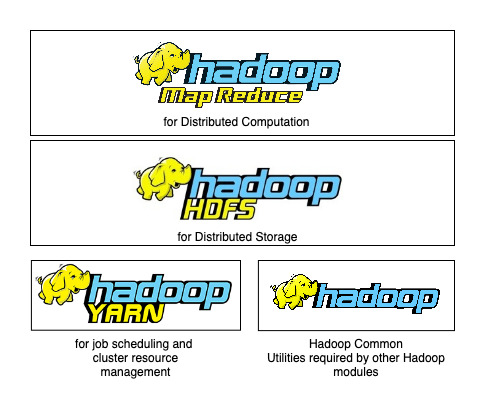
\includegraphics[width=0.9\textwidth]{figures/ch02/hadoop-str}
    \caption{Arsitektur Hadoop}
    \label{fig:hadoop-str}
\end{figure}

\subsection{Mode Kerja Hadoop}
Hadoop dapat dijalankan dalam tiga mode operasi yang berbeda yaitu \textit{standalone, pseudo-distributed}, dan \textit{fully distributed} \cite{johnDataLakeEnterprises2017}. Dalam \textit{standalone mode}, semua proses Hadoop berjalan pada satu node tunggal menggunakan sistem berkas lokal tanpa memerlukan konfigurasi kustom pada Hadoop seperti pada Gambar \ref{fig:hadoop-modes}. 

\begin{figure}[h!]
    \centering
    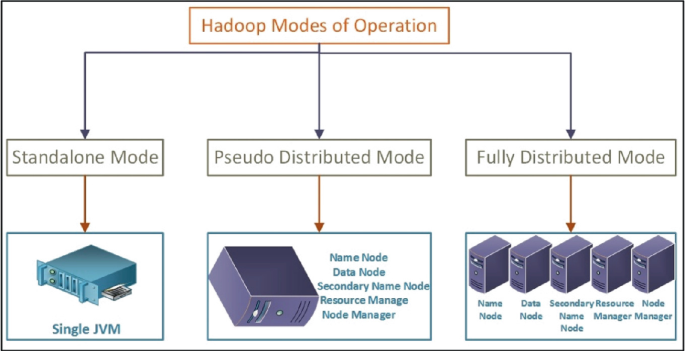
\includegraphics[width=0.9\textwidth]{figures/ch02/hadoop-modes}
    \caption{Mode Kerja Hadoop \cite{khataiImplementationTextMining2021}}
    \label{fig:hadoop-modes}
\end{figure}

\textit{Pseudo-distributed mode} menjalankan semua komponen Hadoop pada satu node tunggal tetapi menyimulasikan kluster dengan komunikasi antar proses melalui socket jaringan, sehingga memerlukan konfigurasi pada berkas \textit{core-site, mapred-site}, dan \textit{hdfs-site}. Sedangkan \textit{fully distributed mode} menyebarkan proses Hadoop ke beberapa node dalam kluster sebenarnya yang biasanya digunakan untuk tahap produksi. \textit{Fully distributed mode} mendukung skalabilitas, ketersediaan tinggi, dan keamanan dengan memerlukan instalasi Hadoop dan konfigurasi kluster pada setiap node.

\subsection{Hadoop Distributed File System (HDFS)}
\textit{Hadoop Distributed File System} adalah sistem file terdistribusi yang dikembangkan sebagai bagian dari Hadoop \cite{abhishekIntegratedHadoopCloud2017}. HDFS dirancang khusus untuk menyimpan data dalam jumlah besar dan memungkinkan pemrosesan data secara paralel. Beberapa fitur utama dari HDFS antara lain skalabilitas, toleransi kesalahan, \textit{streaming access}, dan cocok untuk aplikasi \textit{batch} seperti MapReduce.

\begin{figure}[h!]
    \centering
    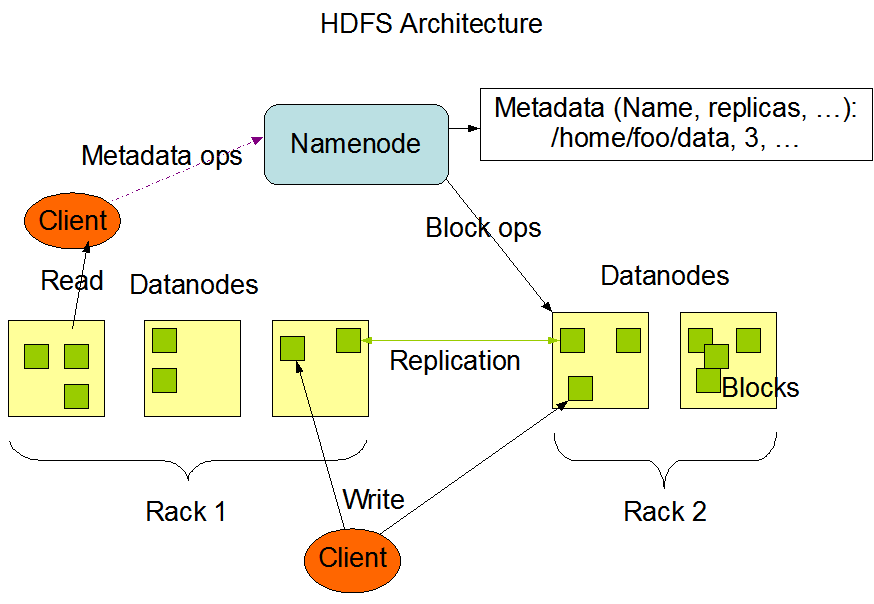
\includegraphics[width=0.9\textwidth]{figures/ch02/hdfsarchitecture}
    \caption{Arsitektur HDFS \cite{ApacheHadoopHDFS}}
    \label{fig:hdfs-arch}
\end{figure}

Secara struktur, HDFS terdiri dari NameNode sebagai \textit{node master} yang mengelola \textit{metadata} dan \textit{namespace}, serta DataNode sebagai \textit{node slave} yang bertugas menyimpan data sebenarnya dalam bentuk blok seperti pada Gambar \ref{fig:hdfs-arch}. Berkas di HDFS dipartisi menjadi satu atau lebih blok berukuran 64MB atau 128MB, kemudian didistribusikan dan disimpan di beberapa DataNode. Setiap block direplikasi (biasanya 3x) di DataNode yang berbeda untuk toleransi kesalahan. Replikasi blok di \textit{node/rack} yang berbeda juga meningkatkan ketersediaan HDFS.

Dengan desain terdistribusi, HDFS sangat populer digunakan bersama framework Hadoop untuk memproses \textit{big data} \cite{almansouriHadoopDistributedFile2019}. Namun, ketergantungan pada \textit{single} NameNode dan performa akses data acak yang kurang optimal menjadi kelemahan utama HDFS. Secara keseluruhan, HDFS telah terbukti menjadi pilihan matang untuk penyimpanan data massal secara terdistribusi.

\subsection{Hadoop YARN}
\textit{Hadoop YARN} (\textit{Yet Another Resource Negotiator}) adalah manajer sumber daya dan sistem penjadwalan untuk kluster Hadoop. Komponen ini diperkenalkan dalam Hadoop 2.x sebagai evolusi dari Hadoop MapReduce 1.x, yang mengintegrasikan manajemen sumber daya dan pemrosesan data dalam satu sistem. YARN memungkinkan kluster untuk menjalankan berbagai aplikasi secara bersamaan dengan efisiensi yang lebih baik.  YARN memisahkan fungsi manajemen sumber daya dari mekanisme pemrosesan data, yang sebelumnya keduanya tertanam dalam MapReduce. Dengan demikian, YARN dapat mendukung berbagai paradigma pemrosesan data di atas Hadoop, selain MapReduce, seperti \textit{real-time processing} dan \textit{graph processing}.

\begin{figure}[h!]
    \centering
    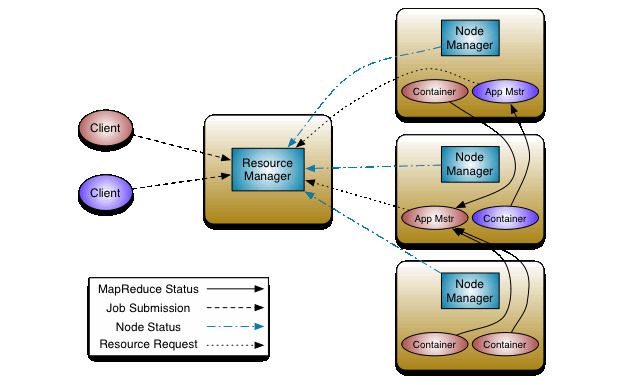
\includegraphics[width=0.9\textwidth]{figures/ch02/yarn-arch}
    \caption{Arsitektur YARN \cite{ApacheHadoopApache}}
    \label{fig:yarn_arch}
\end{figure}

Struktur utama YARN terdiri dari ResourceManager yang bertugas mengkoordinasikan alokasi sumber daya di seluruh kluster, dan NodeManager yang berjalan di setiap \textit{node} untuk mengawasi penggunaan sumber daya dan mengelola \textit{container} tempat aplikasi dijalankan. \textit{ApplicationMaster} adalah komponen khusus untuk setiap aplikasi yang bertanggung jawab untuk negosiasi sumber daya dengan ResourceManager dan bekerja dengan NodeManager untuk menjalankan dan memantau \textit{tasks} seperti pada Gambar \ref{fig:yarn_arch}.

\subsection{Apache Spark}
Apache Spark pertama kali diperkenalkan oleh Apache Software Foundation pada tahun 2014 sebagai \textit{framework} pemrosesan data paralel \textit{open-source} yang dirancang untuk mempercepat pemrosesan \textit{big data} dibandingkan dengan  Hadoop MapReduce \cite{ApacheSparkUnified}. Meskipun sama-sama menggunakan model pemrosesan MapReduce, Spark bukanlah hasil modifikasi dari Hadoop MapReduce\cite{KOMPARASIKECEPATANHADOOP}. Hal ini dikarenakan Spark menggunakan teknologi tersendiri yaitu \textit{Resilient Distributed Datasets} (RDDs) yang memungkinkan Spark memproses data secara \textit{in-memory} sehingga lebih cepat. Menurut laporan resmi, Spark mampu memproses data 10-100 kali lebih cepat dibandingkan MapReduce Hadoop. Selain itu, Spark memiliki klaster pengolahan data tersendiri sehingga dapat berjalan independen tanpa Hadoop. Dengan performa tinggi serta dukungan untuk pemrosesan data secara interaktif, Spark banyak digunakan untuk pemrosesan data skala besar.

\subsection{HiBench}

\subsubsection{Cara Kerja HiBench}

\subsubsection{Sumber Data pada HiBench}

\subsubsection{Beban Kerja pada HiBench}


\section{Penelitian Terkait}

Penelitian terdahulu yang relevan seperti yang ditunjukkan oleh Tabel \ref{table:penelitian-terdahulu} menghasilkan temuan penting mengenai performa sistem pemrosesan data besar. Penelitian oleh Ahmed et al. \cite{ahmedComprehensivePerformanceAnalysis2020} dan Yasir Samadi et al. \cite{samadiPerformanceComparisonHadoop2018} menyoroti perbandingan performa antara Hadoop dan Spark dalam kondisi dan beban kerja yang berbeda. Pada penelitian tersebut, ditunjukkan bahwa meskipun Hadoop dan Spark beroperasi pada prinsip MapReduce, ada perbedaan signifikan dalam cara kedua \textit{software} menangani dan memproses data, terutama dalam hal efisiensi dan penggunaan sumber daya. 

\begin{table}[!htbp]
\centering
\caption{Tabel Perbandingan Referensi}
\label{table:penelitian-terdahulu}
\begin{tabular}{|p{1.5cm}|p{1.25cm}|p{2.75cm}|p{3cm}|p{4cm}|}
\hline
\textbf{Penulis} & \textbf{Tahun} & \textbf{Beban Kerja yang Diuji} & \textbf{Spesifikasi Perangkat Keras} & \textbf{Hasil} \\
\hline
Ahmed et al. \cite{ahmedComprehensivePerformanceAnalysis2020} & 2020 & WordCount and TeraSort (50--600 GB) & SNCC, Production Cluster CPU cores -- 80 Total Storage -- 60 TB Master node -- 1 Slaves nodes -- 9 & Spark memiliki performa yang lebih baik hingga dua kali lipat dalam beban kerja WordCount dan hingga 14 kali lipat dalam beban kerja TeraSort. \\
\hline
Yasir Samadi et al. \cite{samadiPerformanceComparisonHadoop2018} & 2018 & Micro Benchmarks Web Search SQL Machine Learning (1 GB, 5 GB and 8 GB) & VM, Disk(SDD) -- 40 GB & Spark lebih efisien daripada Hadoop untuk menangani data dalam jumlah besar dalam kasus-kasus besar. Namun, Spark membutuhkan alokasi memori yang lebih tinggi. \\
\hline
Satish dan Rohan \cite{gopalaniComparingApacheSpark2015} & 2015 & K-means (62--1240 MB) & VM 2 nodes, 4 GB RAM, 500 GB & Kecepatan Spark hingga tiga kali lebih tinggi dari MapReduce. \\
\hline
\end{tabular}
\end{table}
